\section{Controle Nebuloso e Robótica Evolutiva}

\setcounter{subsection}{-1}
\subsection{Definição dos Consequentes }

O primeiro passo no controle do robô é a definição dos consequentes das regras
que serão levadas em conta. Considerando que o robô dispõe de 3 sensores
(\(d_1\), \(d_2\) e \(d_3\)) e que as funções de pertinência associadas às
medidas realizadas por eles estão representadas na seção 3 do enunciado, sugestões de consequentes estão
representadas na tabela \ref{tab:consequentes}, logo abaixo. As regras são da
forma \textbf{SE (\(d_1\) É x) E (\(d_2\) É y) E (\(d_3\) É z) ENTÃO
(\(\Delta \theta\) É w)}.

				\begin{table}[H]
					\centering
					\caption{\label{tab:consequentes} Regras que controlarão o robô.}
					\setlength\tabcolsep{4pt}
					\begin{minipage}{0.30\textwidth}
					    \centering
						\begin{tabular}{| c | c | c | c |} 
						\hline
						\(d_1\) & \(d_2\) & \(d_3\) & \(\Delta \theta\) \\ \hline
						P & MP & P & MN  \\ \hline
						P & MP & M & MN \\ \hline
						P & MP & G & MN \\ \hline
						P & PP & P & Z  \\ \hline
						P & PP & M & MN \\ \hline
						P & PP & G & MN \\ \hline
						P & PG & P & Z  \\ \hline
						P & PG & M & MN \\ \hline
						P & PG & G & MN \\ \hline
						P & MG & P & Z  \\ \hline
						P & MG & M & PN \\ \hline
						P & MG & G & MN \\ \hline
						\end{tabular}	
					\end{minipage}	      
					\begin{minipage}{0.30\textwidth}
					    \centering
						\begin{tabular}{| c | c | c | c |} 
						\hline
						\(d_1\) & \(d_2\) & \(d_3\) & \(\Delta \theta\) \\ \hline
						M & MP & P & PP \\ \hline
						M & MP & M & MP \\ \hline
						M & MP & G & MN \\ \hline
						M & PP & P & PP \\ \hline
						M & PP & M & Z  \\ \hline
						M & PP & G & PN \\ \hline
						M & PG & P & PP \\ \hline
						M & PG & M & Z  \\ \hline
						M & PG & G & PN \\ \hline
						M & MG & P & PP \\ \hline
						M & MG & M & Z  \\ \hline
						M & MG & G & PN \\ \hline
						\end{tabular}	
					\end{minipage}	
					\begin{minipage}{0.30\textwidth}
					    \centering
						\begin{tabular}{| c | c | c | c |} 
						\hline
						\(d_1\) & \(d_2\) & \(d_3\) & \(\Delta \theta\) \\ \hline
						G & MP & P & MP \\ \hline
						G & MP & M & MP \\ \hline
						G & MP & G & MP \\ \hline
						G & PP & P & MP \\ \hline
						G & PP & M & MP \\ \hline
						G & PP & G & MP  \\ \hline 	  	 
						G & PG & P & MP \\ \hline
						G & PG & M & PP \\ \hline
						G & PG & G & Z  \\ \hline
						G & MG & P & MP \\ \hline
						G & MG & M & PP \\ \hline
						G & MG & G & Z  \\ \hline
						\end{tabular}	
					\end{minipage}	      
			    \end{table}
	\FloatBarrier
	
	\subsection{Controlando o Robô}
	
	Uma vez definidas as regras que deverão ser seguidas, o próximo passo é então
	simular o comportamento do robô através do \textit{software} MATLAB. Para isso,
	5 funções foram escritas. A primeira, chamada \texttt{trap\_pertinencia},
	recebe 6 parâmetros, sendo eles a coordenada \(x\), as informações \(a\), \(b\), \(c\)
	e \(d\) referentes os trapézios que compõem as funções de pertinência e o valor
	a ser considerado caso \(x\) esteja fora do intervalo \(\left[a, d\right]\), e
	retorna o respectivo valor da função de pertinência. O programa
	\ref{lst:trap_pertinencia} abaixo possui a implementação da respectiva
	função.
	
	\lstinputlisting [language=Matlab, caption={ \texttt{trap\_pertinencia.m} -
	Avalia pertinência de um regra em função de \(x\).},
	label={lst:trap_pertinencia}] {fuzzy/trap_pertinencia.m}
	
	\vspace{12pt}
	
	A segunda função, chamada de \texttt{get\_D1\_D3\_Rule} e representada pelo
	programa \ref{lst:d1d3}, calcula a pertinência de cada um dos possíveis estados
	referentes aos sensores \(D_1\) e \(D_3\).	Essa função recebe como parâmetro a
	distância medida pelo sensor e retorna um vetor com três valores contendo a
	pertinência para os estados \textbf{P}, \textbf{M} e \textbf{G}. 
	
	\lstinputlisting [language=Matlab, caption={
	Avalia pertinência da regras de \(D_1\) e \(D_3\) em função das distâncias
	medidas.}, label={lst:d1d3}] {fuzzy/get_D1_D3_Rule.m}

	\vspace{12pt}
	
	A função \texttt{get\_D2\_Rule} realiza o mesmo que o descrito anteriormente,
	mas agora com o sensor \(D_2\). A implementação desta função pode ser
	encontrada logo abaixo.
	
	\lstinputlisting [language=Matlab, caption={
	Avalia pertinência da regras de \(D_2\) em função das distâncias
	medidas.}, label={lst:d2}] {fuzzy/get_D2_Rule.m} 
	
	\vspace{12pt}
	
	A quarta função, \texttt{get\_Angle\_Rule}, implementa as regras descritas na
	tabela \ref{tab:consequentes}. Por ser extensa, a sua implementação foi
	colocada na seção \textbf{Anexos} ao fim deste documento no programa
	\ref{lst:angle_rule}. Em poucas palavras, esta função testa se cada uma das
	regras está ativa e, caso uma determinada regra esteja, atribui a ela o menor
	valor dentre as pertinências dos estados que a compõem. Por exemplo, se \(D_1\)
	é \textbf{P} com 50\%, \(D_2\) é \textbf{MG} com 100\% e \(D_3\) é \textbf{M}
	com 33\%, então \(\Delta \theta\) é \textbf{PN} com 33\%.
	
	\vspace{12pt}
	
	A quinta função, \texttt{get\_Angle}, é responsável pelo processo de
	\textit{defuzzyficação} e está representada pelo programa \ref{lst:angle}. Ela
	utiliza o método de centro de massa para determinar \(\Delta \theta\) que
	melhor convém dadas as regras ativas.
	
	\lstinputlisting [language=Matlab, caption={
	Avalia pertinência da regras de \(D_2\) em função das distâncias
	medidas.}, label={lst:angle}] {fuzzy/get_Angle.m}
	
	\vspace{12pt}
	
	Enfim, a sexta função, \texttt{robot\_control}, realiza o controle do robô
	conforme regras especificadas acima. Sua implementação está representada pelo
	programa \ref{lst:control}.
	
	\lstinputlisting [language=Matlab, caption={  
	Automatiza controle do robô.}, label={lst:control}] {fuzzy/robot_control.m}  
	
	\subsection {Resultados}
	
	A fim de testar o controlador implementado na seção anterior, dois mapas foram
	criados. Os resultados das execuções estão representados na figuras
	\ref{fig:test_fuzzy_1} e \ref{fig:test_fuzzy_2}, em que a trajetória está
	representada em preto, a parede em cinza claro, os pontos de destino em cinza
	escuro e as posições livres, em branco. Para ambos, a direção inicial do robô é
	\(\frac{\pi}{2}\), as coordenadas iniciais são \((3,3)\) e a velocidade é \(v =
	1 \) \textit{pixel/iteração}. Verifica-se que o controle é bem-sucedido, sendo
	que o robô é capaz de realizar as curvas presentes nos mapas. É importante
	comentar que os cantos \textit{suavizados} possuem uma grande importância para o
	bom resultado, uma vez que o controle nas áreas de ``ponta'' não é tão eficiente
	visto que, quando o controlador verifica a proximidade a uma parede, ele pode
	não saber para que lado virar.
		
	\FloatBarrier
			    
	\begin{figure}[h!]
	
	\centering
	
		\begin{subfigure}{.5\textwidth}
		  \centering
		  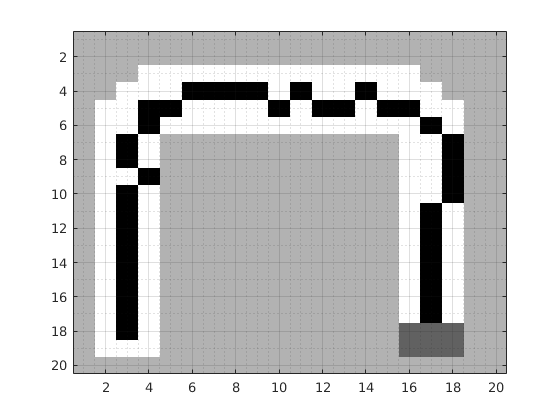
\includegraphics[width=1\linewidth]{fuzzy/test1}
		  \caption{\centering Controle do robô no mapa 1.}
		  \label{fig:test_fuzzy_1}
		  
		\end{subfigure}%
		\begin{subfigure}{.5\textwidth}
		  \centering
		  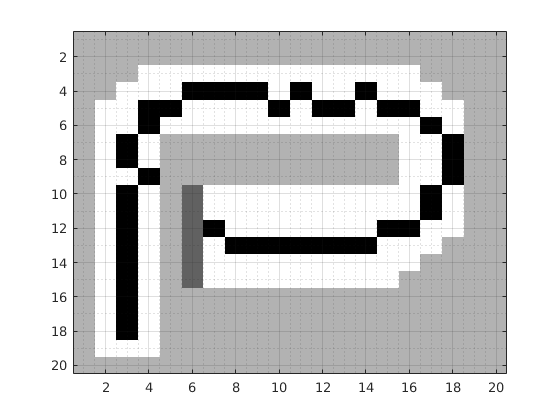
\includegraphics[width=1\linewidth]{fuzzy/test2}
		  \caption{\centering Controle do robô no mapa 2.}
		  \label{fig:test_fuzzy_2} 
		\end{subfigure}
	
	
	\caption{Resultados para o controle nebuloso do robô
	para dois mapas distintos.}
	\end{figure} 
	
	\FloatBarrier
		
	O \textit{script} utilizado nos testes pode ser encontrado no programa
	\ref{lst:test_fuzzy}.
	
	\lstinputlisting [language=Matlab, caption={  
	\textit{Script} de teste..}, label={lst:test_fuzzy}]
	{fuzzy/test_robot_control.m}

	\subsection {Controle via Rede Neural MLP}
	
	A adaptação do controle do robô via redes neurais exigiu algumas modificações
	nos programas fornecidos anteriormente nesta seção e também no algoritmo de
	evolução fornecido pelo professor, que foi utilizado na seção \ref{sec:pid}.
	Foram utilizados, neste caso, \(N = 10\) para a camada intermediária, 100
	gerações e 100 indivíduos na população.
	
	\vspace{12pt}
	
	Para o algoritmo evolutivo, foram alteradas a função de \textit{fitness}, a
	estrutura do cromossomo e as taxas de mutação e \textit{crossover}, conforme
	explicado a seguir.
	
	\begin{itemize}
	  \item A função de \textit{fitness} utilizada foi
	  \(f_{fitness}=\frac{1}{n_{colisao} + 1}\). Logo, soluções que obtiverem
	  muitas colisões serão piores, isto é, terão um \textit{fitness} menor. A
	  linha adicionada ao código foi, portanto:
	  
\begin{lstlisting}[language=Matlab, style=nonumbers]
fitness(i,1) = 1/(colision_i + 1);
\end{lstlisting}
	
	  \item  Anteriormente, tínhamos apenas 3 parâmetros a evoluir, sendo eles
	  \(k_d\), \(k_p\) e \(k_i\). Neste caso, o número de parâmetros depende do
	  número de neurônios na camada intermediária. Sejam \(N\) neurônios nesta
	  camada, cada um deles terá 4 pesos, sendo um deles para a entrada constante e
	  o restante para as distâncias dos sensores. Há ainda mais \(N + 1\) pesos a
	  serem ajustáveis, correpondentes à soma dos resultados de cada neurônio. A
	  estrutura utilizada foi, portanto:
	  
\begin{lstlisting}[language=Matlab, style=nonumbers]
% Numero de entradas: d1, d2, d3 e termo constante
E = 3 + 1;
pop = randn(tam_pop, E * n_neurons + n_neurons + 1);
\end{lstlisting}	  
	
	  Utilizou-se também uma distribuição normal de média 0 e variância 1 para os
	  pesos iniciais da rede neural.
	  
	  \item A fim de maximizar a diversidade na rede, utilizou-se taxas de mutação
	  \(p_m = 0.8\) e \textit{crossover} \(p_c = 0.9\).

	\end{itemize}
	
	O controle do robô, realizado pela \texttt{robot\_control\_mlp}, também foi
	alterado. A linhas referentes ao controle nebuloso (linhas 75 a 86 do programa
	\ref{lst:control}) foram retiradas e substituídas pelo trecho de código abaixo.
	
\begin{lstlisting}[language=Matlab, caption={Trecho de código do controle do
robô feito via rede MLP.}, label={lst:control_mlp}] 
% Constroi vetor das entradas de cada neuronio
mlp_input = [distance_d1 distance_d2 distance_d3 1];

% middle_layer_output contera as saidas de cada neuronio da camanda
% intermediaria
middle_layer_output = zeros (1, n_neurons);

% Calcula a saida de cada neuronio. mlp_weights contem todos os pesos
% sinapticos da rede 
for n = 1 : n_neurons
    
    middle_layer_output (1, n) = ...
        tanh(mlp_input * mlp_weights (1 + (n - 1)* 4 : 4 + (n - 1)* 4)');
    
end

% a entrada da ultima camada eh a saida da camada intermediaria e uma
% termo constante.
last_layer_input = [middle_layer_output 1];

% Calcula o desvio na direcao do robo. Seleciona ultimos n_neurons + 1 pesos
% sinapticos. 
d_angle = ...
 last_layer_input * mlp_weights (1 + 4 * n_neurons : 1 + 4 * n_neurons + n_neurons)';

robot_direction = robot_direction + d_angle;

teste (round(m_length + 1 - y_robot), round(x_robot)) = 'r';

% Calcula nova posicao.
x_robot = x_robot + speed*cos(robot_direction);
y_robot = y_robot + speed*sin(robot_direction);

% Verifica se a nova posicao esta dentro do mapa.
if (round(x_robot) > length(labyrinth_matrix (1,:))) ...
        || (round(x_robot) < 1) ...
        || (round(m_length + 1 - y_robot) < 1) ...
        || (round(m_length + 1 - y_robot) > m_length)
    
    % Penalisa movimentos que levam o robo fora do mapa.
    colisions = colisions + 1000;
    
% Detecta colisao.
elseif (labyrinth_matrix (round(m_length + 1 - y_robot), round(x_robot)) == '#')
    
    % Aumenta contador de colisoes.
    colisions = colisions + 1;
end
\end{lstlisting}
	
O mapa da figura \ref{fig:test_fuzzy_2} foi utilizado no treinamento da rede
neural, visto que apresenta situações mais desafiadoras que o mapa da figura
\ref{fig:test_fuzzy_1}. Sendo assim, acredita-se que se o programa for
bem-sucedido em calcular os pesos sinápticos para o mapa mais complexo, então,
os mesmos pesos serão adequados para mapas mais simples. As figuras
\ref{fig:mlp_2} e \ref{fig:mlp_1} contém resultados para um dos vetores de
pesos sinápticos encontrado pelo algoritmo evolutivo em que essa afirmação é
comprovada.

\FloatBarrier
			    
	\begin{figure}[h!]
	
	\centering
	
		\begin{subfigure}{.5\textwidth}
		  \centering
		  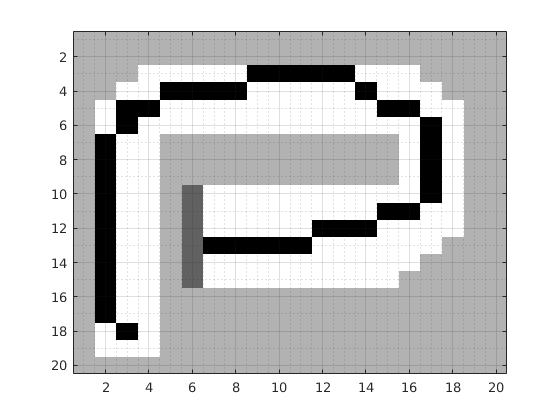
\includegraphics[width=1\linewidth]{mlp_robot/mlp_2}
		  \caption{\centering Controle do robô via MLP no mapa 2.}
		  \label{fig:mlp_2}
		  
		\end{subfigure}%
		\begin{subfigure}{.5\textwidth}
		  \centering
		  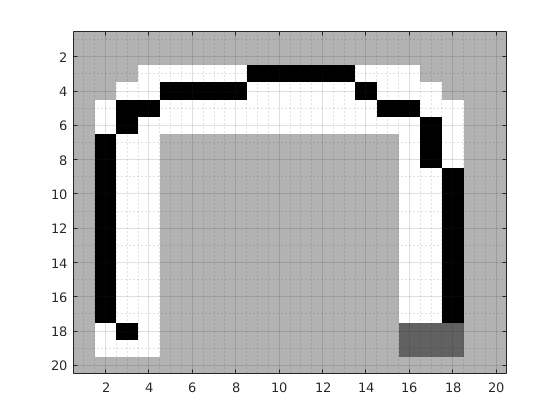
\includegraphics[width=1\linewidth]{mlp_robot/mlp_1}
		  \caption{\centering Controle do robô via MLP no mapa 1}
		  \label{fig:mlp_1} 
		\end{subfigure}
	
	
	\caption{Resultados para o controle do robô via MLP
	para dois mapas distintos.}
	\end{figure} 
	
	\FloatBarrier
	
	A figura \ref{fig:fitness_mlp} representa a evolução do \textit{fitness} ao
	decorrer da execução do algoritmo evolutivo. Verifica-se que, apesar da melhor
	solução ser encontrada nas primeiras gerações, o \textit{fitness} médio é muito
	pequeno em todas as gerações. Esse fato pode ser explicado pelos valores das
	taxas de mutação e \textit{crossover}, responsáveis por manter uma grande
	diversidade na população. Dessa forma, sempre serão adicionados à população
	indivíduos ruins, isto é, que produzem baixos \textit{fitness}.
	
	\FloatBarrier
	
	\begin{figure}[h]
    \centering
    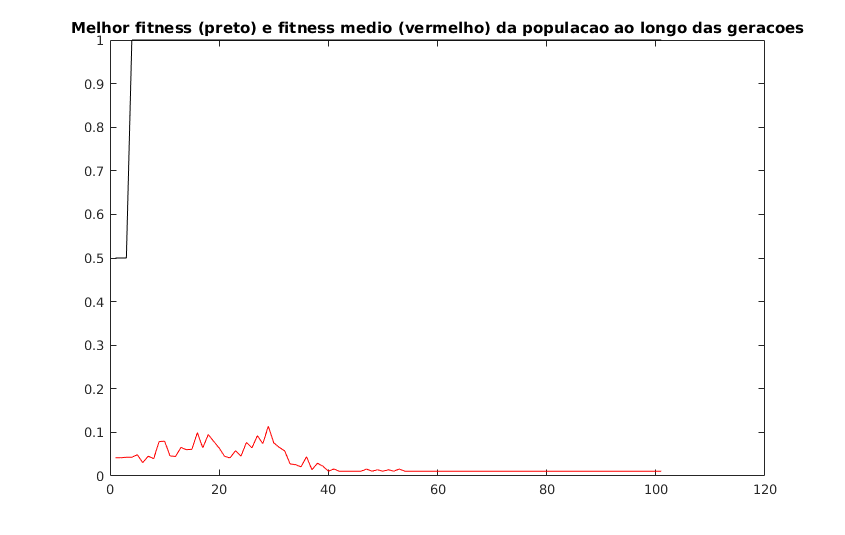
\includegraphics[scale=0.65]{mlp_robot/fitness}
    \caption{\label{fig:fitness_mlp}Evolução do \textit{fitness} médio e
    melhor.}
	\end{figure}  
	
	\FloatBarrier
	
	As figuras \ref{fig:mlp_2_1} e \ref{fig:mlp_2_2} foram obtidas pelo
	treinamento da rede neural no mapa da figura \ref{fig:test_fuzzy_1}.  
	
	\FloatBarrier
			    
	\begin{figure}[h!]
	
	\centering
	
		\begin{subfigure}{.5\textwidth}
		  \centering
		  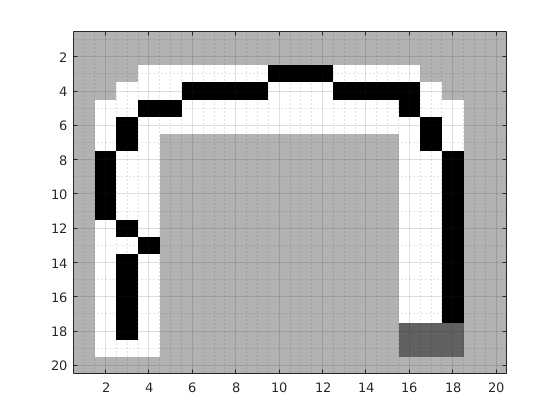
\includegraphics[width=1\linewidth]{mlp_robot/mlp_1_2}
		  \caption{\centering Controle do robô via MLP no mapa 1.}
		  \label{fig:mlp_2_1}
		  
		\end{subfigure}%
		\begin{subfigure}{.5\textwidth}
		  \centering
		  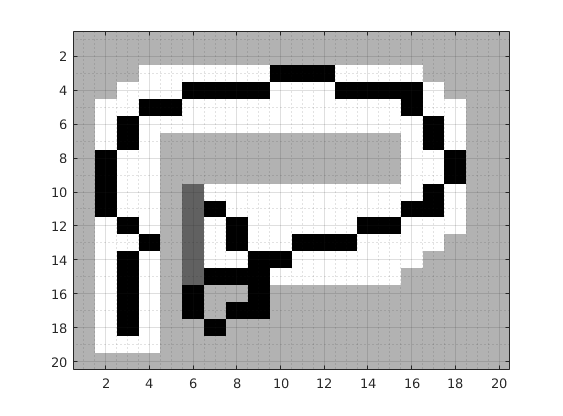
\includegraphics[width=1\linewidth]{mlp_robot/mlp_2_2}
		  \caption{\centering Controle do robô via MLP no mapa 2.}
		  \label{fig:mlp_2_2} 
		\end{subfigure}
	
	
	\caption{Resultados para o controle do robô via MLP
	para dois mapas distintos.}
	\end{figure} 
	
	\FloatBarrier
	
Verifica-se que a solução encontrada para o primeiro mapa, que é mais simples,
controla corretamente o robô. Entretanto, se o mesmo controle fosse utilizado
para o mapa 2, então o robô colidiria com a parede, conforme mostrado na figura
\ref{fig:mlp_2_2}. Isso é explicado pelo fato de que o mapa exige um controle
mais complexo que o primeiro.
